\documentclass[10pt, a4paper]{article}
\usepackage{lrec2006}
\usepackage{lingmacros}
\usepackage{graphicx}
%\usepackage[utf8]{inputenc}

\title{Combining Language Resources Into A Grammar-Driven Swedish parser}

\name{Malin Ahlberg, Ramona Enache}

\address{ Department of Computer Science \& Engineering\\
          Gothenburg University \\
          Box 8718, SE-402 75 Gothenburg, Sweden\\
          ahlberg.malin@gmail.com, enache@chalmers.se \\}


% 150-200 words here
\abstract{This paper describes work on a rule-based, open-source parser for
Swedish. The central component is a wide-coverage grammar implemented in the GF
formalism (Grammatical Framework), a dependently typed grammar formalism
based on Martin-L{\"o}f type theory. GF has strong support for multilinguality and
has so far been used successfully for
controlled languages \cite{cnl} and recent experiments have showed
that it is also possible to use the framework for parsing free language.
In addition
to GF, we use two other main resources: the Swedish treebank Talbanken and the
electronic SALDO lexicon. By combining the grammar with
a lexicon extracted from SALDO we obtain a parser accepting all sentences
described by the given rules. We develop and test this
on examples from Talbanken.
The resulting parser gives a full syntactic analysis of the input sentences.
It will be highly reusable, freely available, and as GF provides libraries for
compiling grammars to a number of programming languages, chosen parts of the the 
grammar may be used in various NLP applications. 
\\ \newline \Keywords{GF, Swedish, Parsing}}

\begin{document}

\maketitleabstract


\section{Introduction}
% Copied from Master's Thesis. ok to do that?
Our goal is to implement a wide-coverage grammar and parser for Swedish
using the GF formalism, and 
thereby investigate how GF can be used for open-domain parsing.
We compile a large-scale grammar to a parser
and combine it with the extensive lexicon SALDO. The Swedish treebank 
Talbanken provides manually tagged trees which we use for improving and evaluating
the grammar. The parser will additionally
be evaluated by experts. \\
We chose our resources so that both our grammar and parser can 
be freely available and open-source. 
The target language is Swedish, a North-Germanic language
closely related to Norwegian and Danish. The languages share most of their
grammatical structures and are mutually intelligible. Swedish is also 
one of the official languages in Finland and altogether spoken by approximately 9
million people.
Swedish syntax is often similar to English, but the  morphology is richer and the
word order slightly more intricate.
It is a verb-second language: the second constituent of a declarative main
clause must consist of a verb.
The first constituent of the clause is usually made up of the subject,
although it likewise could consist of adverbial phrases or objects.
Fronting the finite verb marks questions.

This paper will briefly introduce GF, Talbanken and SALDO in Section \ref{sec:background}
Section \ref{sec:extractsaldo} explains how we extract a lexicon, section \ref{sec:mapping}
how we translate Talbanken to GF annotation and section \ref{sec:grammar}
presents the work on the grammar implementation.


\section{Background}
\label{sec:background}
\subsection{Grammatical Framework}
\label{sec:gf}


Grammatical Framework \cite{ranta-2011} is a grammar formalism based on
functional programming. 

The key idea is to divide a grammar into abstract and concrete parts. 
The abstract grammar gives a logical representation of the semantics,
modeled as abstract trees.
The concrete grammars tell how to translate the abstract trees to a given language,
and deal with issues such as word order, case and agreement. 
The framework enables us to parse strings into abstract trees as well as
linearize trees into strings.

The grammar acts as an independent module and reusability is further supported
by the separation between resource grammars and application grammars. The
resource library provided with GF implements morphological and syntactical
rules for more than 20 different languages.  Hence the writer of an application
grammar can start her work at a higher level and does not need to describe how
to form standard sentences, phrases or inflect words.

Since many of the languages in the GF library resemble each other grammatically,
they can share much of their implementations. This is usually done by using a
\verb|Functor| by which we avoid code duplication and which aids the code maintenance.

GF has so far been used in a number of projects,
MOLTO\footnote{http://www.molto-project.eu/}, TALK \cite{talk}
and WebAlt \cite{webalt} to mention a few. 
All those are special domain applications, dealing with controlled natural
language.
This project takes a different approach by using GF for open domain language,
as done in recently conducted work on translating patents \cite{patent}.

Using the Swedish resource grammar as our starting
point, we get a basic description of the language. The framework provides
tools such as parsing, generation and
a well-tested interpretation of the parse trees. Furthermore, there are tools
for using GF grammars in a number of programming languages like Haskell
and Java. 



\subsection{Talbanken}
For development and evaluation, we use the Swedish treebank
Talbanken \cite{talbanken}.
It was assembled in the 1970s at Lund University and modernized
in 2005 \cite{talbanken05} and
enriched with annotation for a full phrase structure analysis.  \\
Although Talbanken contains both written and spoken Swedish,
only the prose material, consisting of 6316 sentences, is used in this
project.
This part was also used when training the data-driven parser Maltparser \cite{malt}. \\

\subsection{SALDO}
SALDO \cite{saldo} is an open source lexicon resource
based on Svenskt Associationslexikon. It is
developed at Spr{\aa}kbanken at Gothenburg University
and intended for usage in language technology
research. 
We have developde tools for extracting GF lexicons
from SALDO, described in \ref{sec:extractsaldo}
%which have resulted in a dictionary containing
%over 98000 entries including information about verbs that
%are reflexive or needs a particle.
%The importing method should be fast and reliable
%enough to allow us to always have a fresh version of the dictionary
%in GF.

\section{Related work}
%Copied form thesis!!!! 
% Add: how are these related to this work?
% Add :detaild comparison of outputs of various parsers of Sw.
Many years of research have lead to many interesting language
technology tools for Swedish.
An example is the well-known data-driven Malt parser \cite{malt},
trained on Talbanken. 
There are also a number of grammar-based parsers, although none is freely available.
The cascaded finite state parser CassSwe \cite{casswe} and
The Swedish Constraint Grammar \cite{birn}
give syntactic analyses. 
Swedish FDG (Voultanien,2001) uses the Functional Dependency Grammar
\cite{fdg},
an extension of the Constraint Grammar
formalism, and produces a dependency structure focusing on finding the nominal
arguments. \\

The LinGO Grammar Matrix \cite{matrix}, is a starter-kit for building
Head-Driven Phrase Structure Grammars \cite{hpsg} (HPSG) providing
compatibility with tools for parsing, evaluation, semantic representations etc.
Translation is supported by using Minimal Recursion
Semantics \cite{mrs} as an interlingua. 
There is a collection of grammars implemented in this framework, giving broad-coverage
descriptions of 
English, Japanese and German. 
The Scandinavian Grammar Matrix \cite{scandmatrix} covers common parts of
Scandinavian, while Norsource (Hellan, 2003) describes Norwegian. A Swedish version
was based upon this by Ahrenberg, covering the morphology and some
differences between Swedish and Norwegian. Further, there is the BiTSE 
grammar \cite{stymne}, also implemented using the Lingo Matrix,
which focuses on describing and translating verb frames.\\ 


The Swedish version of the Core Language Engine (CLE) \cite{gamback}
gives a full syntactic analysis as well as semantics represented in `Quasi logical form'. A
translation to English  was implemented and the work was further developed in the spoken
language translator \cite{spoken}. Unfortunately, it is no longer available. The coverage of the Swedish
CLE is also reported to be very limited \cite[p. 134]{nivreTrees}.\\

In the TAG formalism \cite{tag}, there are projects on getting open source, wide-coverage grammars
for English and Korean, but, to our knowledge, not for Swedish.  \\

The ParGram \cite{pargram} project aims at making wide coverage grammars using
The grammars are implemented in parallel in order to coordinate the analyses of
different languages and there are now grammars for English, German, Japanese and Norwegian. 

%old related work:
%Language technology for Swedish is an area of much interesting research.
%There are two other deep grammar-based parser for Swedish:
% put in references!!
%Swedish Core Language Engine (Raynen and Gambäck, 1992) and a
% does this really exist??
%unification-based chart parser \cite{wiren},
%though none of them are freely available.
%Among other parsers for Swedish, the statistical MaltParser \cite{malt},
%trained on Talbanken, is worth mentioning. 
% put in references!!
%CassSwe (Kokkinakis and Johansson-Kokkinakis, 1999) is based on finite state cascades,
% put in references!!
%whereas the shallow parser GTA (Knutsson, Bigert and Kann, 2003) relies on rules of 
%a context free grammar. Both GTA and CassSwe operate on POS tagged text.\\
%Extract and FM \cite{MarkusForsberg2007} are tools for supervised lexicon
%extraction compatible with GF.

%\section{Results and progress}
%\label{sec:progress}

\section{Extracting a large lexicon}
\label{sec:extractsaldo}
The lexicon provided with the GF resources is far too small for open-domain
parsing.
This section describes the process of importing SALDO, which is 
compatible with GF, and easily translated to GF format.
As SALDO is continuously updated, the importing process has been designed to be fast
and stable enough to be redone at any time.

\subsubsection{Implementation}
The basic algorithm for importing SALDO was implemented by Angelov (2008)
and  produces code for a GF lexicon.
For each word in SALDO, it decides which forms should be used as input
to the GF smart paradigms. The smart paradigm is a function which given one
form of a word, can infer which paradigm it most likely belongs to.
For verbs, this will in most cases mean giving
the present tense form, see figure \ref{fig:saldoknyt}. \\

\begin{figure}[h]
\begin{center}
\verb-mkV "knyter" ;-
\includegraphics[scale=0.5]{image1.eps} 
\caption{First code produced for the verb `knyta' (\emph{`tie'})}
\label{fig:saldoknyt}
\end{center}
\end{figure}

All assumed paradigms are printed to a temporary lexicon, 
which will produce an inflection table for every entry when compiled.
The tables are compared to the information given
in SALDO and if the tables are equal the code for the word is saved. If the table
is erroneous, another try is made
by giving more forms to the smart paradigm.
For example \ref{fig:saldoknyt}, the smart paradigm will fail to calculate the
correct inflection table. In the next try both the present and the past tense
are given:\\

\begin{figure}[h]
\begin{center}
\verb-mkV "knyter" "knöt" ;-
\caption{Second output for the verb `knyta'}
\label{fig:saldoknyt2}
\end{center}
\end{figure}

The program is run iteratively until the GF table matches the one given in SALDO,
or until there are no more ways of using the smart paradigm. The verb 'knyta'
will need three forms:\\

\begin{figure}[h]
\begin{center}
\verb-mkV "knyter" "knöt" "knutit"-\\
\caption{Final output for the verb `knyta'}
\label{fig:saldoknyt3}
\end{center}
\end{figure}


\subsubsection{Results}
\label{sec:saldoRes}
The resulting dictionary contains more than 100 000 entries, approximately 80 \% 
of the total size of SALDO.
There are a number of reasons why some words were not imported,
the most obvious one is that we do not want all categories from
SALDO in the GF lexicon. Prepositions, 
numerals, 
personal pronouns etc.
are assumed to be present in the resource grammars and should not be added again.
SALDO contains many pronouns which
are not analysed the same way in GF. %TODO see where??
Before adding them to our lexicon, we need to do more analysing to find their
correct GF-category. 
%Some experiments on finding the category
%have been done using Talbanken, see section \ref{sec:gf.quant}.
Categories involving multiple words 
are usually handled as idioms and should be given in a separate lexicon. In
total six types of words were considered for the extraction: \\

\begin{figure}[h]
\begin{tabular}{|l|ll|}
\hline
& SALDO$/$GF & Example \\
\hline
 Adverb & \textbf{ab}$/$\textbf{Adv} & ofta (\emph{often})\\
 Adjective&\textbf{av}$/$\textbf{A} & gul (\emph{yellow})\\
 Noun & \textbf{nn}$/$\textbf{N} & hus (\emph{house})\\
 Verb & \textbf{vb}$/$\textbf{V} & springa (\emph{run})\\
 Reflexive verbs &\textbf{vbm}$/$\textbf{V} & raka sig (\emph{shave})\\
 Particles verbs &\textbf{vbm}$/$\textbf{V}  &  piggna till (\emph{perk up})\\
\hline
\end{tabular}
\caption{}
\end{figure}

Most but not all words of these categories have been imported.
One reason why the importing phase would fail 
is that SALDO, unlike GF, only contains the actually used word forms.
For technical reasons, the smart paradigm might need forms never used.
Consider for example the plural tantum 
noun \emph{`glas{\"o}gon'} (\emph{`glasses'}).
The smart paradigm requires a singular form, and since the program could not
find this in SALDO, there was no way of adding the lemma to the lexicon. 
When the program failed to import a noun, this was often the explanation.
Words of this type may be added manually, for \emph{`glas{\"o}gon'} we could use
the ostensibly correct singular form `glas{\"o}ga', although this
has another meaning (`glass-eye').
The same problem occurred for the irregular s-verbs,
(\emph{`synas'} \emph{(`show')} or \emph{umg{\aa}s} \emph{(`socialize')})
which made up 61.5 \% of the failing verbs of type \verb_vb_.\\
In a few cases the smart paradigms could not generate the correct declination.\\

When testing the coverage of Talbanken,
we found that there are around 2500 word forms still missing, excluding the ones
tagged as names and numbers. This number may seem very high, but 
4/5 of the word forms are compounds and when performing the intended parsing,
an additional analysis identifying compounds is preformed before
looking-up the words in the lexicon. We
should also take into consideration that 
we cannot automatically find out how many actually stem from the same word, or
how many abbreviations that are present. Talbanken also contains a small number of 
spelling errors, which probably are enumerated among our missing words. The majority
of the missing words are only used once.\\

\begin{figure}[h]
\begin{tabular}{|l|l|}
\hline
Missing words &$\sim$ 2500 word-forms\\
\hline
\hline
Ignoring compounds & $\sim$ 500 word-forms\\
Used more than once & $\sim$ 500 word forms\\
Used more than once,& \\
\hspace{2mm} ignoring compounds & $\sim$ 150 word-forms\\
\hline
\end{tabular}
\caption{}
\end{figure}

A list of words that were given different labels in GF than in Talbanken has been
composed, consisting of about 1600 entries. Many of those are
acceptable and reflects the difference 
made in the analyses, while
others are examples of words that are still missing from
the lexicon.

%Since SALDO does not give any valency information, neither does the imported lexicon.
%The lexicon does not contain any information.
\noindent Valency information, which is crucial for GF, is not given in SALDO and
hence not in the imported lexicon. Instead we extract this from
Lexin\footnote{http://spraakbanken.gu.se/lexin/}.


\subsection{A tool for lexical acquisition}
As we extract our main lexicon from SALDO, we have also created a tool for
semi-automatic acquisition to complement the lexicon.
%We have tested it on verbs, with good results.
Like the SALDO importer it makes use of
the smart paradigm given in the Swedish resource grammar.
Unlike the SALDO importer, this tool does not require any particular
word form, but operates on any verb form and 
%By combining this method with the information from the tags in Talbanken,
%the tool interactively generates GF lexical entries. 
%Given a list of words, it 
iteratively tries to figure out how to conjugate each of them. If several forms
of a word are 
given, the program will try to identify the one that carries the most linguistic
information, put this in a form recognized by the smart paradigm and ask GF to output
a table with the resulting inflection. 
If the table contains all other conjugations from the input list,
the program will ask the  user to
validate the claimed paradigm. 
This step is needed since the input may not provide information enough
to automatically do the validation. The user may now either
allow the word to be added to the lexicon, remove it or request another guess.
The user hence only needs to decide if each paradigm is correct or not, and
the program will do the rest.

The tool has been tested on verbs. Although using simple techniques it 
manages to assign the correct paradigm to 70-75 \% of the given lemmas.
A smaller test has shown that out of the accepted lemmas, the correct guess is
made directly in 75\% of the cases, whereas the user has to reject one or more
guesses for 25\%. 
%Hence the program gets a correctness rate of 56 \% if it is
%run without help from the user. This kind of use is however not intended,


%add: ?
%From this a lexicon with about 1000 verbs have been extracted, manually verified.


\section{Translating The Treebank Talbanken}
\label{sec:mapping}
The information from the tags in Talbanken can be used for many purposes.
We have developed an automatic transformation of Talbanken trees 
to trees in GF format. The translation makes use of the POS tags as well as
the syntactic information. 
\begin{figure}[h!]
\begin{center}
\hspace{-30mm}
\subfloat{\label{pic:tbtree}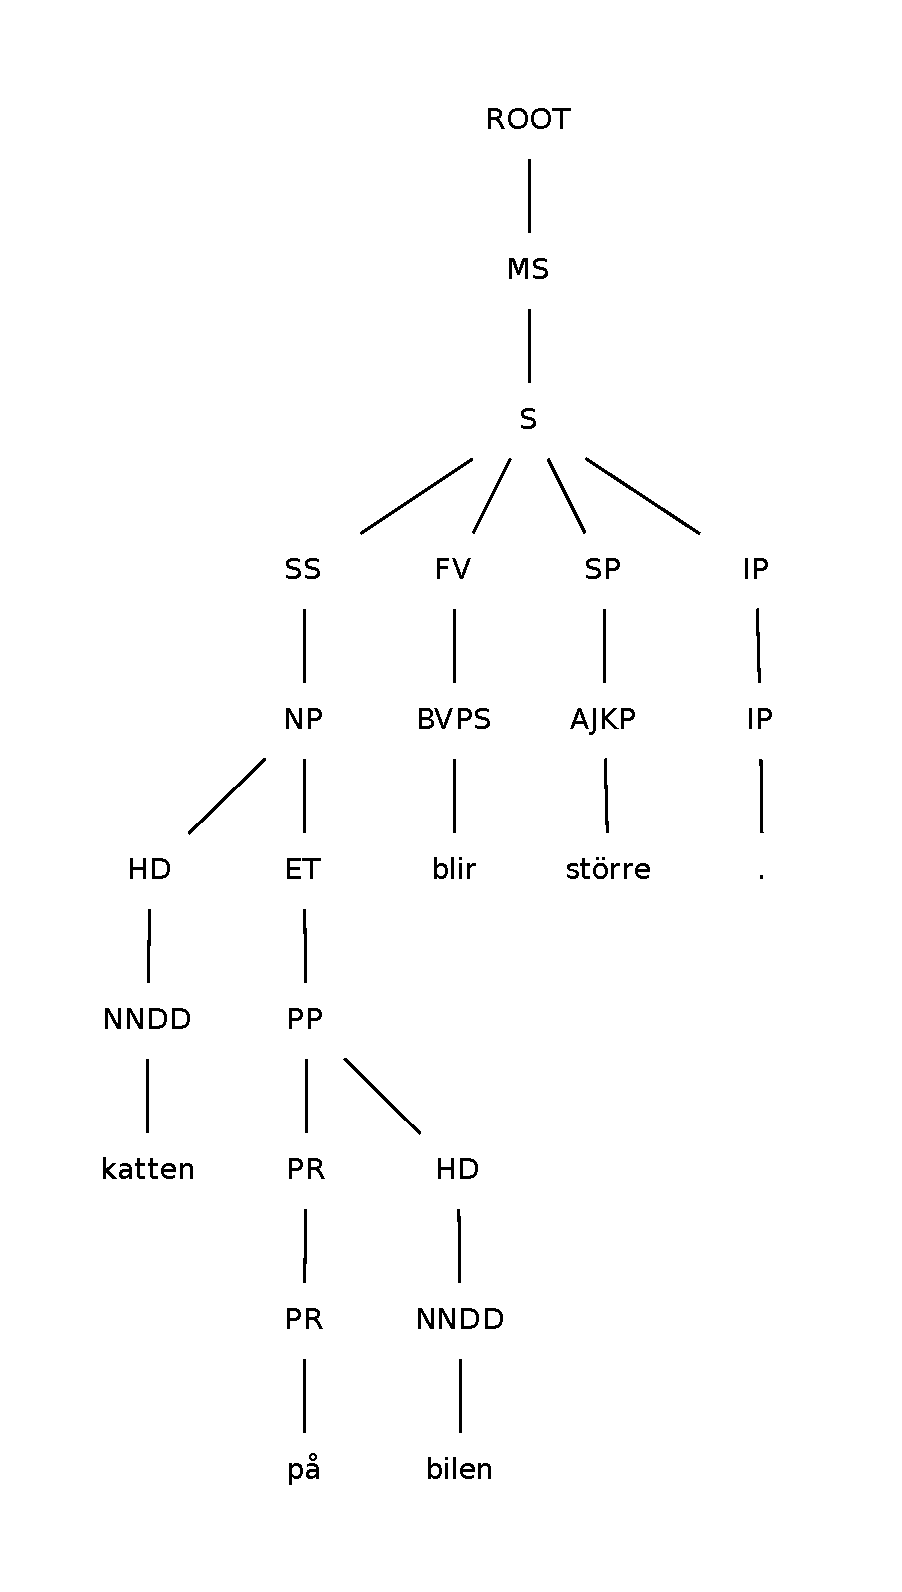
\includegraphics[width=60mm]{Talbankentree.pdf}}
\hspace{-10mm}
\subfloat{\label{pic:gftree}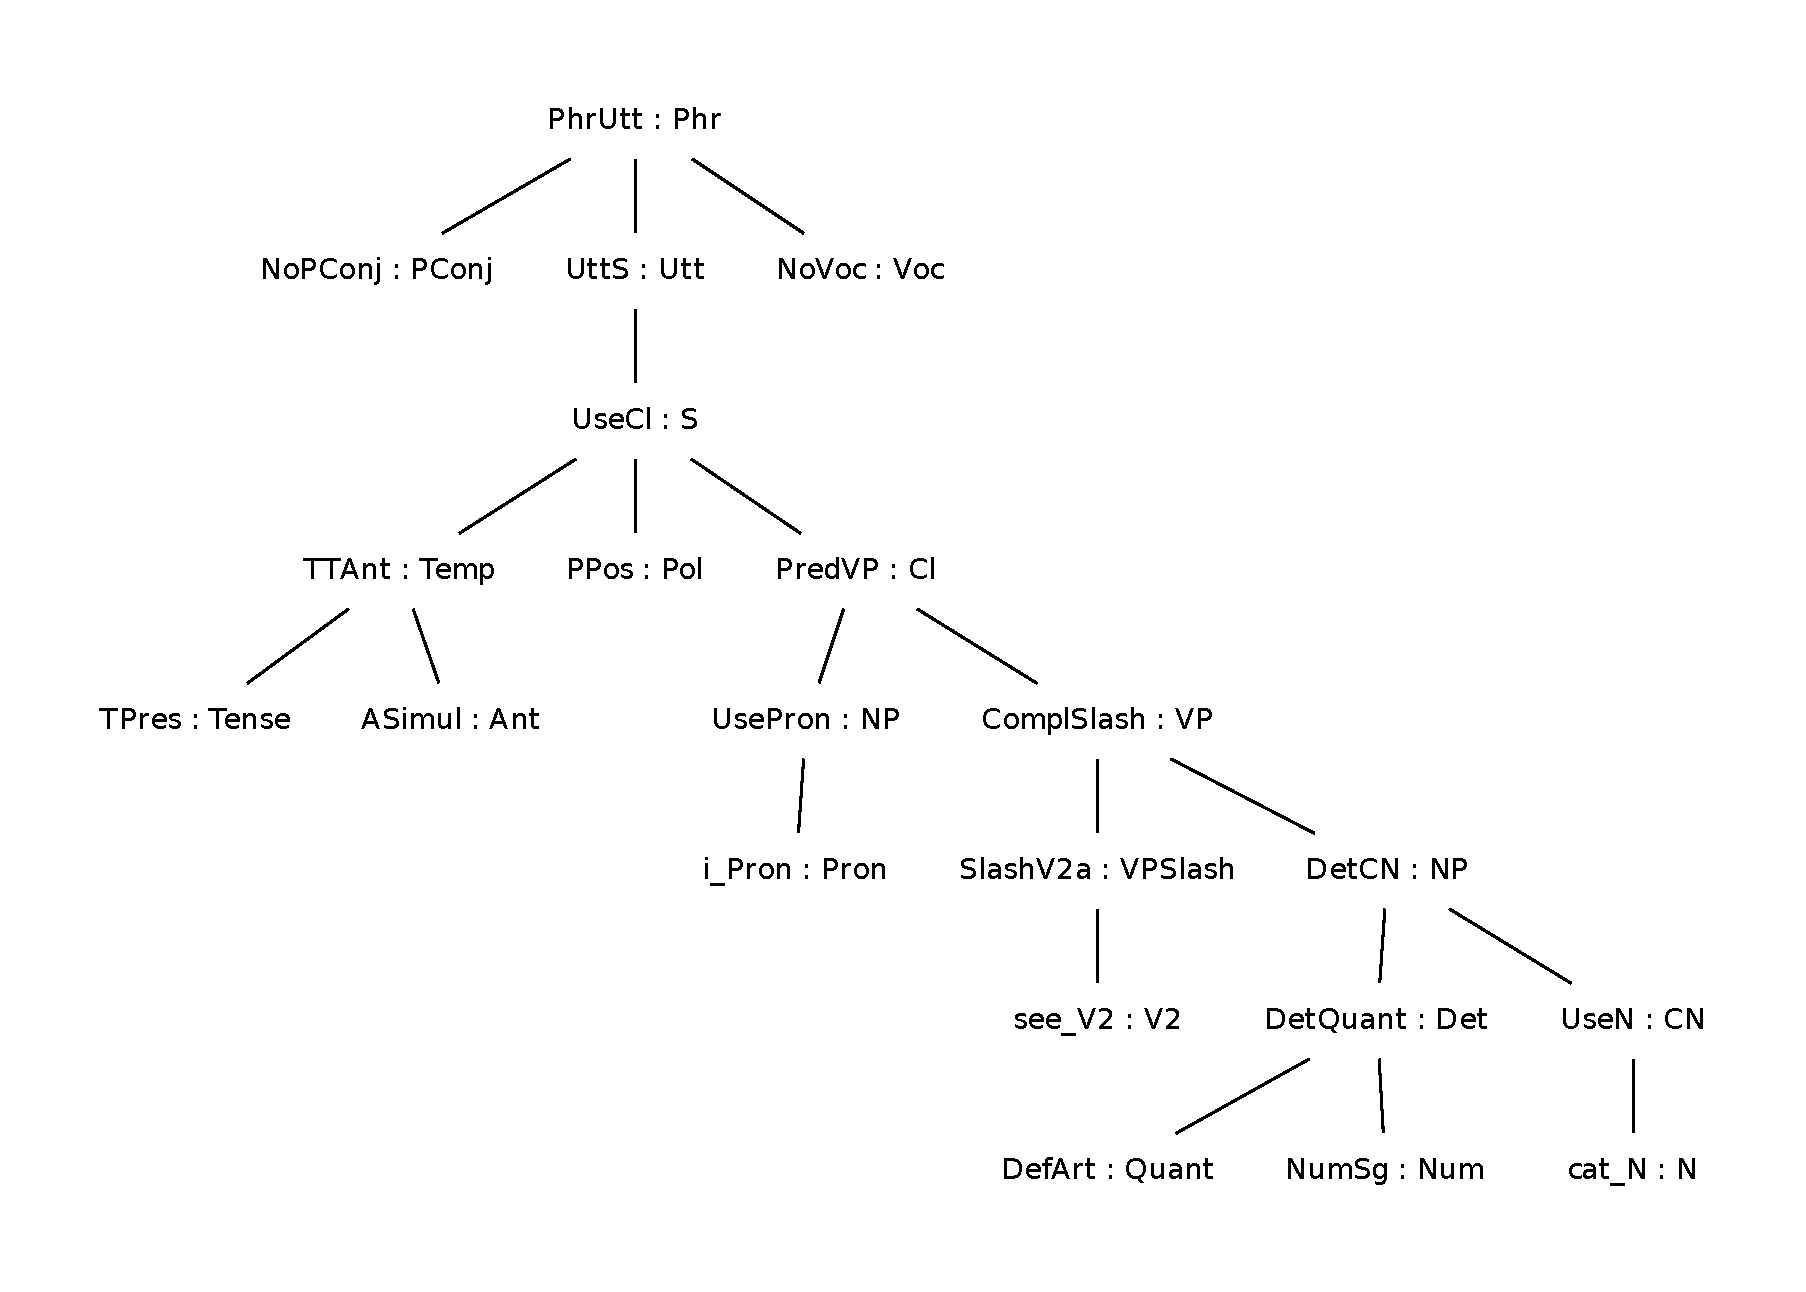
\includegraphics[width=90mm]{gfTree.pdf}}
%\subfloat{\label{pic:gfptree}\includegraphics[width=50mm]{gfPTree.pdf}}
\caption{The Talbanken tree and the GF tree for the sentence ``Katten p{\aa} bilen blir st{\"o}rre".}
\label{fig:translationtrees}
\end{center}
\end{figure}


Figure \ref{fig:translationtrees} shows an example of a visualized Talbanken05 tree
of the sentence ``Katten p{\aa} bilen blir st{\"o}rre" 
(\emph{``The cat on the car gets bigger"}).
The mapping is based on 
a translation of the English Penn Treebank \cite{gfpenn}.
By modifying this program, we now have a translation that works for
the Tiger XML-format of
Talbanken. Adaption was required for the differences in annotation as well as 
for the syntactic differences between Swedish and English.

The translation %connects GF with another annotations and 
gives us means to evaluate our parser. By both parsing a Talbanken sentence and
transforming its annotated tree, we can easily inspect if the results are
equal.
Additionally, the mapping shows which grammatical constructions that are still missing
from the GF grammar and shows how the GF analysis differs from the one made
in Talbanken.
If there are words missing from our dictionary, the rich
POS-tags may help us to automatically find the correct declination and add it to the
lexicon. Further, our parser will need probabilities of how often a function is
used. The GF treebank we achieve from the translation is a good source for this
information.\\

%The mapping gives information about which form a word is
%currently used in and this may be used by the lexical extraction
%tools.
%The translated trees enable us to extract probabilities for how often
%different functions are used, a feature that will enable disambiguation.
%Furthermore, the translation makes it easy to identify grammatical constructions
%missing from the GF grammar and shows how the GF analysis differs from the one made
%in Talbanken.
%Another important use of the mapping is evaluation of the parser, which can be
%accomplished by comparing the parse trees and the trees from the transformer.
%\subsection{Differences in the notation}
%Some structural differences between GF and Talbanken became obvious during the
%translation.
%In Talbanken the valency information is given implicitly by the complements
%of a word. If a verb is followed by an object, \verb-OO-, which contains an
%\verb-S-, we can conclude that this is a sentence-complement verb.
%In GF, the valency information is given for each entry in the lexicon.
%A sentence-complement verb has the type \verb-VS- and from this we know 
%that the function \verb-ComplVS- should be used to combine the verb and with a 
%sentence.
%\begin{wrapfigure}{l}{0.52\textwidth}
%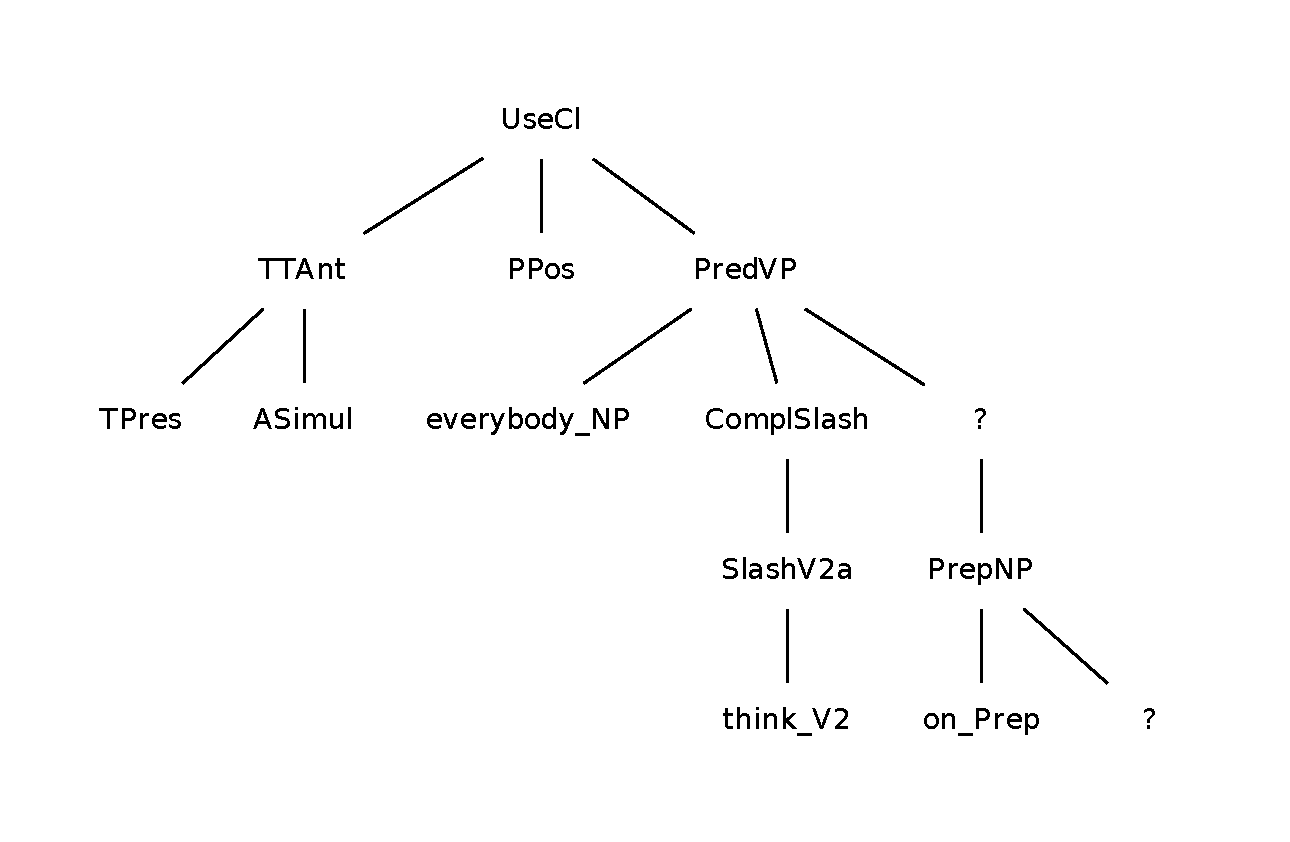
\includegraphics[width=80mm]{metatree.pdf}
%\caption{Abstract tree with meta variable}
%\label{pic:gMetatree}
%\end{wrapfigure}
%
%\noindent A similar issue arises from the use of verb particles. A verb with a
%particle is treated as two independent units in Talbanken but in GF they are
%considered to be one constituent. % which means that 
%The particle has therefore no effect on the abstract tree, its presence is
%announced by the verb \\itself.
%
%
%We have so far concentrated on shorter sentences, without idioms and
%conjunction. 
%Since GF demands information 
%that is not given by the Talbanken tags -- such as the valency of verbs -- a
%full translation requires that all words used are already known to GF. 
%The evaluation of trees of this sort shows that the mapping
%can restore 85\% of the nodes. 
%If we lift the restrictions, we can restore 63\% of the tags.
\subsection{Results and evaluation}
%>> more! replace words, how much better results (both grammar and mapping) 
%>> more results
%>> motivation, why so bad??\\
The development was mostly example-driven, and at least one rule for the translation of
every Talbanken-tag has been implemented.
Shorter sentences have been prioritized in order to get a coverage of the most
fundamental constructions. 
Regression testing was used to ensure that a new rule would not violate the old ones
or allow trees to be translated erroneously.


The flat version of Talbanken05 was used for developing the mapping, but
the program works for both the flat and the deep Tiger-XML versions.
%The deeper contains six more tags, although they are not always useful for our       
%purpose. Figure \ref{fig:mappDeepFlat} shows the difference for a conjunction.
%% show piece of s5 here!
%\begin{figure}[h]
%\begin{parsetree}
%    ( .CNP. 
%        (.CJ.  (.NP. ~ `oskifta dödsbon'))
%        ( .++. (.++OC. `och'))
%        (.CJ.  (.VN. `familjestiftelser'))
%    )
%\end{parsetree}
%\begin{parsetree}
%    ( .CNP. 
%        (.CJ.  (.NP. ~ `oskifta dödsbon'))
%        ( .CC.
%            (.CNP. 
%                (.++.  (.++OC. `och' ))
%                (.C+.  (.VN. `familjestiftelser'))
%         ))
%    )
%\end{parsetree}
%\caption{An example of the difference in the two analyses}
%\label{fig:mappDeepFlat}
%\end{figure}
The focus on the mapping has been simple sentences, in order to cover the most
fundamental structures. 
%If the program is extended and adapted to cover complex
%conjunction, a deeper evaluation should be preformed to see which version that
%suits our needs the best.
%The deeper implementation also gives 
%some more information about verb phrases, by the tag \verb|VG| (\emph{verb group}),
%which groups an infinitival verb and its object together into a \verb|VP|.
%This information can however be extracted from the flat implementation, and the results
%get slightly better when using this version. \\


When evaluating the mapping, the results strongly depend on which restrictions we
put on the input. 
One of the reasons why a node cannot be translated, is the 
use of the tags show in figure \ref{fig:mapBadtag}.
The \textbf{PU} tag is used for graphic listings, and not for fluent text.
In our grammar there is naturally no corresponding function; 
%We are not interested in sentences made up by list, since 
the listings are meant for making the text look nice in
folders etc and outside the scope for the grammar itself. The tags \textbf{XX}
and \textbf{NAC} are often used since Talbanken makes a
difference between subject
and object noun phrases. %(which is not needed in GF (see section \ref{sec:swegf}))
The analysis of elliptical expression in (\ref{sent:krav})
\enumsentence{F\"or stora krav.\\
``Too high demands."}\label{sent:krav}
contains the tags \textbf{XX} and \textbf{NAC}, since it is not obvious
whether the noun phrase is used as subject or an object.
The tags shown in figure \ref{fig:mapBadtag} occur quite frequently in the treebank and are always translated
to metas, which lowers our result. \\
%How we cannot cover all cases. 
\begin{figure}[h]
\begin{tabular}{ll}
\textbf{NAC} & Not a constituent\\
\textbf{XP} & Other (non-coordinated) phrase\\
\textbf{DB} & Doubled function\\
\textbf{PU} & List item\\
\textbf{XX} & Unclassifiable part-of-speech\\
\end{tabular}
\caption{}\label{fig:mapBadtag}
\end{figure}


The main goal has been to be able to translate shorter sentences, with no
idioms or conjunction.
If we assure that the lexicon contains the correct word class for all lemmas
involved, we
can restore more than 85 \% of the nodes in the original tree.
If we lift all the restrictions excluding the \verb|PU|, we get
%When tested the 100 first sentences from Talbanken, we get
65 \% coverage. 
If we test randomly collected sentences that do not contain any of the tags listed
in figure \ref{fig:mapBadtag}, 72 \% can be restored (see figure \ref{tab:mappres})

%TODO
%All NPs: 72%
\begin{figure}[h]
\begin{tabular}{|ll|}
\hline
No list items & 65 \%\\
No special punctuation or bad tags& 72 \%\\
Short sentences with known words & 85 \%\\
\hline
\end{tabular}
\caption{}
\label{tab:mappres}
\end{figure}

A mapping between GF and the Wall Street Journal of Penn Treebank has earlier been conducted \cite{gfMech}.
The percentage of restored nodes from Peen Treebank is higher than our results.
%TODO review
The reason for this may be the fact that English is syntactically less complicated
than Swedish.
Furthermore, the text in Talbanken are from various brochures, newspapers and text books,
where idiomatic expressions are more likely the be appear and the language
presumably less strict than in Wall Street Journal\footnote{www.wsj.com}.
Also, the Penn Treebank contains a lower number of tags, 82 compared
to more than 300 in Talbanken. Even if the tags describing the same word
%TODO review
class as another tag are excluded, Talbanken still leaves us with more than 130 tags.
With more tags, we get more information, but as the number 
%Thus the number of
increase, so does the amount of work of finding the correct translation 
for each combination of tags and writing rules that cover all constructions. 
%iand so is the number of
%rules that would be needed to cover all constructions.

We believe that the results could be enhanced by simply adding more rules 
and in this way get a wider coverage. There are many special cases that require
special rules. Since we are not aware of any formal specification of how the tags may be
combined in Talbanken, the only way of finding all possibilities are to manually look
for different patterns. Another option would be to make the mapping more
robust, but the robustness must not interfere with the correctness.


\section{Development of the grammar}
\label{sec:grammar}
An important part of this project has been to develop the Swedish GF grammar and
to adapt it to cover constructions used in Talbanken. As a grammar
implementation can never be expected to give
full coverage of a language, we aim for a grammar fragment which gives a deep
analysis of the most important Swedish constructions.
The starting point has been the GF resource grammar and the new implementation is
still compatible with this.

It has earlier been hard to identify missing constructions of the Swedish
implementation, since there was no large resource available to evaluate it on.
Our evaluations are based on Talbanken, and when first conducting tests,
we found much room for improvement.
%For Swedish, about 85\% of the GF resource code is shared with the other Scandinavian
%languages. 
%However, if we aim for a deeper and more comprehensive analysis of Swedish,
the implementation of the languages needs to be more independent.
The resource grammar gives a good start and our present grammar 
% don't say inverted word order
covers constructions such as declarative sentences, questions, passives,
imperatives, relative clauses, cleft constructions etc.
During our work the grammar has been extended to cover language specific
constructions such as topicalisation and the features listed below. We further
put effort on avoiding and removing overgeneration, which might pass unnoticed
when parsing controlled text but which cause an explosion of ambiguous parse trees
when used for free text and with a large lexicon.
\subsection{The s-passive}
Passive voice is commonly used in Swedish.
There are two ways of forming passive verb phrases in Swedish: the 
\textbf{periphrastic passive}, formed by using the modal auxiliary verb `bli'
(\emph{`become'}) and the \textbf{s-passive} which is formed by adding an
\emph{s} to the verb: \\
\enumsentence{
\shortex{5}{Uppsatsen & skrev\textbf{s} & av & en & student.}
        {\emph{the essay} & \emph{wrote+\textbf{s}} & \emph{by} & \emph{a} & \emph{student}}
        {``The essay was written by a student."}}\label{sent:skrevs}
%{b. &En & student & skrev & uppsatsen.}
%        {&a &student &wrote &the essay}
%        {~~`A student wrote the essay.'}}
Some studies suggest that the s-passive is used in more than 80 \% of the times
\cite{laanemets}.
It is however not as common in the other Scandinavian languages,
and the resource grammar for Scandinavian therefore only implemented a function for
passive by using auxiliary verb.

During this project, the s-passive was added and the
periphrastic passive is still allowed.
The grammar further allows not only two-place verbs, but all verb phrases missing an object, to 
form passive:
\enumsentence{\textbf{Active use of two-place verb}\\\shortex{4}
{Vi & erbj{\"o}d& henne& jobbet }
{\emph{we} & \emph{offered}& \emph{her}&\emph{the job}}
{``We offered her the job"}}
\label{sent:give2pass}
\enumsentence{\textbf{First place in two-place verbs}\\\shortex{3}
{Hon & erbj{\"o}ds & jobbet}
{\emph{she} &\emph{ offered+\textbf{s}}&\emph{ the job}}
{``She was offered the job"}}
\label{ex:passV33}
\enumsentence{\textbf{Second place in two-place verbs}\\\shortex{3}
{Jobbet & erbj{\"o}ds & henne }
{\emph{the job} & \emph{offered+\textbf{s}}&\emph{ her}}
{``The job was offered to her"}}
\label{ex:passV32}
\enumsentence{\textbf{V2A verb}\\\shortex{3}
{Huset & m{\aa}lades & r{\"o}tt}
{\emph{the house} & \emph{painted+\textbf{s}}& \emph{red}}
{``The house was painted red"}}
\label{ex:passV2A}

\subsection{Impersonal constructions}
\label{sec:Formal}
Formal subjects \cite[\textsection 19]{SAG} are often used in
Swedish.
\enumsentence{\shortex{6}
{Det & sitter & en & f{\aa}gel & p{\aa} & taket}
{\emph{it }& \emph{sits }& \emph{a} & \emph{bird} &\emph{ on} & \emph{the roof}}
{``There is a bird sitting on the roof''}}
\emph{`Det'} has the position of the subject, and the real subject, 
\emph{`en f{\aa}gel'} the one of an object.

Our grammar implementation allows impersonal constructions 
and does not allow ungrammatical variants such as sentence
(\ref{sent:fagelfron}) where a transitive verb is used.

\enumsentence{\shortex{5}
{Det&dricks&mycket & {\"o}l& nuf{\"o}rtiden}
{\emph{It}&\emph{drinks+s}&\emph{much} &\emph{ beer}&\emph{ nowadays}}
{``A lot of beer is being drunk these days"}}

The grammar also respects the restrictions on the real subject, which cannot
contain a determiner requiring the noun or modifying adjective to be definite form \cite{Cooper}
\enumsentence{\shortexnt{6}
{*Det     & sitter     & \textbf{den}& \textbf{f{\aa}geln}& p{\aa}       & taket.}
{\emph{it}& \emph{sits}& \emph{the}  & \emph{bird}    & \emph{on}& \emph{the roof}}
}
\enumsentence{\shortexnt{6}
{*Det& sitter& \textbf{min}& \textbf{f{\aa}gel}& p{\aa}& taket}
{\emph{it}&\emph{sits}&\emph{my}&\emph{bird}&\emph{on}&\emph{the roof}}
}\label{sent:dumfagel}
 
\subsection{Formalizing the rules for reflexive pronouns by using dependent types}
\label{sec:reflexives}
An important area in a Swedish grammar is the treatment of the reflexive pronouns and
the reflexive possessive pronouns.
The reflexives require an antecedent with which they agree in
number and person.
Our grammar accept the following sentences:

\enumsentence{Han s{\aa}g sina barns skor.\\ \label{ex:ReflGen}
He saw {\sc self's} children's shoes.}
\enumsentence{Sina vantar hade han gl{\"o}mt p{\aa} t{\aa}get.\\
{\sc self's} gloves, he had forgotten on the train.}
\enumsentence{Hon ber alla sina kompisar att g{\aa}\\
She asks all {\sc self's} friends to leave}\label{ex:ReflPredet}
\enumsentence{Jag vill att han rakar sig.\\
I want him to shave {\sc self}.}
%\enumsentence{\begin{tabular}[t]{@{}*{5}{l@{\ }}} 
%a. & Han är längre än sin kompis. & & b. &Han är här oftare än sin kompis.\\
%   & He is taller than {\sc self's} friend.
%   & & & He is here more often than {\sc self's} friend.
%\end{tabular}}\label{ex:ReflAP} \label{ex:ReflAdv}
\eenumsentence{
\item Hon tyckte om skolan och alla sina elever.\\
     She liked the school and all {\sc self's} students.
\item Han s{\aa}g sina f{\aa} b{\"o}cker och sin penna.\\
 He saw {\sc self's} few books and {\sc self's} pencil.
}\label{ex:ReflConj} \label{ex:ReflConj2}
Reflexive pronouns can not be used in subject noun phrases of finite sentences,
as shown by the ungrammatical examples in 
sentence (\ref{sent:sesig}) and (\ref{ex:ReflSubj}).
The third person reflexives (`sig',`sin') requires a third person antecedent (see \ref{ex:refljag}).
Furthermore, the antecedent must be within the same finite sentence as the reflexive
pronoun, see (\ref{sent:sesig}).
The grammar does not accept any of these sentences:
\enumsentence{
*Sina vantar var kvar p{\aa} t{\aa}get.\\
{\sc self's} gloves were left on the train.}\label{ex:ReflSubj}
\enumsentence{*Han och sin kompis läser en bok.\\
He and {\sc self's} friend are reading a book. }
\enumsentence{*Jag ger sina pengar till sina syskon.\\
I give {\sc self's} money to {\sc self's} siblings. }\label{ex:refljag}
\enumsentence{*Han vill att jag ser p{\aa} sig.\\
He wants me to look at {\sc self}.}\label{sent:sesig}

In order to achieve a scalable implementation of reflexive pronouns, we needed
to diverge from the old abstract implementation. To capture the agreement
between the antecedent and the reflexive pronoun, while still allowing the grammar
to accept reflexive constructions embedded in abverbial and adjectival phrases,
in fronted positions etc. we make use of the dependent types of GF. This is the
first use of the dependent types in the resource grammars and a could be
extended to other languages having similar dependecies.

\subsection{A second future tense: ``Kommer att"}
Swedish use two auxiliary verbs for future tense \\
\cite[p. 246]{H&H}:
%\cite[Tempus \textsection 28]{SAG}.
\eenumsentence{
\item {
Det \textbf{kommer att} bli m{\"o}rkt snart\\
``It will get dark soon" }
\item {
Jag \textbf{ska} g{\aa} och l{\"a}gga mig nu\\
``I'm going to bed now"\\}
}
The resource grammar included 
\emph{`ska'}, which was implemented as the standard way of forming future
tense, and hence represents the translation of
\emph{`will'}. 
The new grammar also supports \emph{``kommer att"}, expressed as an alternative
future tense.
\begin{figure}[h]
\begin{verbatim}
(UseCl (TTAnt TFutKommer ASimul) PPos 
       (ImpersCl (AdvVP (ComplVA become_VA 
                (PositA dark_A)) soon_Adv))
\end{verbatim}
\caption{Result of parsing ``Det kommer att bli m{\"o}rkt snart". The future tense
         is marked by the constant TFutKommer}
  \label{fig:kommeratt}
\end{figure}

\subsection{Testing}
Throughout the project regression testing has been used. Every time the grammar was updated
it was tested against a treebank consisting of 155 sentences, and the number of
parse trees were compared to a standard.
The purpose was first of all to
make sure that the coverage was not decreased, but also to make sure that we
would notice if new ambiguities or overgenerating functions were introduced.
If so, the ambiguities could be removed when possible, and when not, we were made
aware of them and could decide whether the increase of coverage were worth the
increase in ambiguities.

New functions were also tested by random generating and by creating tables showing
all forms of the added construction.

\section{Evaluation and Future Work}
The project has so far resulted in
\begin{itemize}
\item a large-scale GF lexicon and a program to redo the importation when needed
\item an extended grammar covering an important part of Swedish
\item a comparison between GF and another annotation
\item a deeper testing of the Swedish resource grammar and an estimation
%TODO lexin, chunking?
of how well GF can be used to describe larger parts of a language
\item a study of how dependent types can be used in the resource grammars
\end{itemize}

Besides being capable of reimporting SALDO, the lexicon extraction program could also
be modified for importing other lexical resources. The only requirement is that
the resource provides inflection tables.

The grammar has been extended and enhanced, and its current status is
a specialized extension of the resource grammar.
Besides parsing, the grammar may well be used for language generation,
which works fast even when using an extensive lexicon.
Although it is not been formally verified, we believe that the majority of the
sentences generated are grammatically correct in a syntactical point of view.
Without any semantic knowledge, nonsense phrases cannot be avoided in
random generation. However, given that the abstract tree has a meaningful
interpretation,
the linearization should be correct.

When it comes to parsing, we do not get far without robustness.
The grammar in itself is by no means robust, and just one 
unexpected punctuation mark, unknown word
or ellipsis will cause the parsing of the whole sentence to fail. 

Parsing bigger parts of Talbanken would hence give very low results at this stage, 
%, for the reasons stated.
and a comparison of the results would not be of much value as
there would not be enough material %underlag is yet too small 
to do be able to do any interesting analysis.

Without methods for robust parsing, %TODO evaluate??
it is not interesting to talk about coverage, but about the quality and
the ability to scale up, which has so far proved to be good.
We further believe that the presence of a expert in Swedish, professor Elisabet
Engdahl\footnote{http://svenska.gu.se/om-oss/personal/elisabet-engdahl},
has increased the standard substantially.\\

By the renewed import of SALDO, we have doubled the size of the lexicon and thereby
added many of the commonly used words that were missing from the older
version. This is of course a big improvement.
However, the lexical part still requires some work before it can be made use of.
The lexicon is too big to use with the current techniques. Its size causes the
incremental parsing algorithm to use more heap memory than normal computers
allow. To solve this, we need to use the lexicon data more cleverly.

We are currently working on chunk parsing and disambiguation using probabilities
extracted from our translation of Talbanken. We combine this with simple named
entity recognition and compounding analysis. For evaluation, we intend to use
10 \% of Talbanken, chosen so that is does not infer with our test data.

%\section{Evaluation and future work}
%We are building a parser which is based on grammatical rules rather than
%statistics. The parser will therefore validate that
%a given sentence is grammatically correct according to the rules defined.
%Chosen parts of the parser or grammar may be used in other applications
%which deal with controlled natural languages. Automatic language
%generation from the grammar is also provided by GF.
%
%%TODO already done?
%We aim to make the parser robust by equipping it with techniques such as chunk
%parsing, named entity recognition and methods for handling unknown 
%grammatical constructions such as idioms and ellipses. 
%It is already possible to add probabilities for GF functions,
%which rank the parse trees.
%By adding dependency probabilities, we aim to improve the
%potential for disambiguation.

%Use 10 \% of Talbanken as evaluation material, not seen by grammar developer.
The result will be evaluated both automatically -- by comparing the output of
the translated trees from Talbanken -- and manually by professor Elisabet Engdahl.
She also evaluates the intermediate results.

% Add: valencies extracted, compounds from språkbanken
\section{Conclusion}
We have developed the main components
for a deep Swedish parser; an extended grammar and lexicon and material for
evaluation and disambiguation.
By starting from the GF resource grammar, we got a well-defined system for
describing language. 

We have implemented a grammar covering an important fragment of Swedish by
focusing on constructions that are frequent in Talbanken.
\\

All parts of the project are open-source and may thus be used in other applications.
The grammar and the lexicon may be beneficial also when working with controlled languages,
as it increases the coverage of the Swedish resource grammar.

The constructions
that we have focused on have all been possible to implement, with varying  amounts
of work. Many of them could be done by utilizing and extending the resource library
but in some cases we needed to part from the multilingual abstract and use other
grammatical theories in order to arrive at a good analysis.


%By combining GF with a large lexicon, we acquire a deep parser for 
%Swedish. All parts, including the underlying grammar, are open-source and can be re-used.
%We have developed tools for extending the lexicon with words from Talbanken,
%and we show how to make use of the information in the manually tagged
%treebank.
The usage of GF allows us to start from
a well-defined system for describing grammar, as well as tools for
parsing.

\section{Acknowledgments}
We would like to thank Center of Language Technology for funding this project.
Further, special thanks to Aarne Ranta,
Elisabet Engdahl, Krasimir Angelov, Olga Caprotti, Lars Borin and John Camilleri for their help
and support.
%\nocite{*}

\bibliographystyle{lrec2006}
\bibliography{FinBib}

\end{document}

